\documentclass[aspectratio=169,11pt]{beamer}
\usepackage[T1]{fontenc}
\usepackage[utf8]{inputenc}
\usepackage{lmodern}
\usepackage{amssymb,amsmath,booktabs,array,tikz,listings}
\usetikzlibrary{arrows.meta}
\definecolor{ink}{HTML}{19263B}
\definecolor{accent}{HTML}{5C5199}
\definecolor{pale}{HTML}{E9E5F4}
\definecolor{edge}{HTML}{60758B}
\setbeamercolor{normal text}{fg=ink,bg=white}
\setbeamercolor{structure}{fg=accent}
\setbeamercolor{frametitle}{fg=ink,bg=pale}
\setbeamercolor{title}{fg=ink}
\setbeamercolor{footline}{fg=edge}
\setbeamerfont{frametitle}{size=\large,series=\bfseries}
\setbeamersize{text margin left=9mm,text margin right=9mm}
\setbeamertemplate{navigation symbols}{}
\setbeamertemplate{itemize items}[circle]
% Explicit total so pagination works even when the preview has no Beamer .nav file.
% Update this when adding or removing frames.
\newcommand{\sessionframetotal}{63}
\setbeamertemplate{footline}{\hfill\scriptsize\insertframenumber/\sessionframetotal\hspace{9mm}\vspace{3mm}}
\setbeameroption{hide notes}
% To compile a presenter copy, replace the line above with:
% \setbeameroption{show notes}
\lstset{language=R,basicstyle=\ttfamily\small,keywordstyle=\color{accent}\bfseries,
 stringstyle=\color{accent},showstringspaces=false,columns=fullflexible,
 keepspaces=true,breaklines=true,frame=none}
\newcommand{\activity}[1]{{\small\color{accent}\bfseries #1}\par\medskip}
\newcommand{\network}[2][]{%
\begin{tikzpicture}[x=0.8cm,y=0.8cm,actor/.style={circle,draw=accent,fill=pale,thick,minimum size=7mm,inner sep=0pt,font=\small\bfseries},tie/.style={draw=edge,thick,#1}]
\node[actor] (A) at (0,1.8) {A};
\node[actor] (B) at (2,1.8) {B};
\node[actor] (C) at (1,0) {C};
\node[actor] (D) at (3.8,0) {D};
\node[actor] (E) at (3.8,1.8) {E};
\node[actor,fill=gray!12] (F) at (5.6,0) {F};
\foreach \a/\b in {#2}{\draw[tie] (\a) -- (\b);}
\end{tikzpicture}}
\title{Social Network Analysis}
\subtitle{Session 2: Connectivity, centrality, and social position}
\author{Petro Tolochko}
\institute{University of Vienna\\Advanced Data Analysis III}
\date{2026}

\newcommand{\ones}{\mathbf{1}}
\newcommand{\Atoy}{\begin{pmatrix}0&1&1&0&0&0\\1&0&1&0&0&0\\1&1&0&1&0&0\\0&0&1&0&1&0\\0&0&0&1&0&0\\0&0&0&0&0&0\end{pmatrix}}
\newcommand{\disto}{\begin{pmatrix}0&1&1&2&3&\infty\\1&0&1&2&3&\infty\\1&1&0&1&2&\infty\\2&2&1&0&1&\infty\\3&3&2&1&0&\infty\\\infty&\infty&\infty&\infty&\infty&0\end{pmatrix}}


\begin{document}

\begin{frame}{Social Network Analysis}

\titlepage

\note{0--2 min. Welcome. Build directly on the first class. All small networks are synthetic. The core session is 180 minutes including a 15-minute break. Appendix slides are optional.}

\end{frame}

\begin{frame}{What we will explain today}

\begin{itemize}
\item How matrix multiplication describes indirect connections.
\medskip\item How connectivity changes the meaning of centrality.
\medskip\item Why degree, reach, brokerage, and prestige give different rankings.
\medskip\item How to calculate and check these measures in R.
\end{itemize}

\note{2--4 min. Explain that students need sums and matrix multiplication, not prior eigenvalue theory. Eigenvectors will be introduced through a repeated calculation.}

\end{frame}

\begin{frame}{Recall: the adjacency matrix}

With rows as senders and columns as receivers,
\[A_{ij}=1\text{ if }i\to j,\qquad A_{ij}=0\text{ otherwise.}\]
\[\mathbf{k}^{\mathrm{out}}=A\ones,\qquad
\mathbf{k}^{\mathrm{in}}=A^{\mathsf T}\ones.\]
\begin{itemize}
\item $\ones$ is a column vector of $n$ ones.
\item In an undirected graph, $A=A^{\mathsf T}$.
\item The order of actors must agree in every matrix and vector.
\end{itemize}

\note{4--8 min. Ask what A times a column of ones does. Matrix-vector multiplication is a set of row sums here. Reintroduce transpose explicitly.}

\end{frame}

\begin{frame}{Our six-person network}

\begin{columns}[c]
\column{.54\textwidth}\centering\network{A/B,A/C,B/C,C/D,D/E}
\column{.43\textwidth}\[A=\Atoy\]
\end{columns}\medskip
Node order: A, B, C, D, E, F. Ties are undirected.

\note{8--12 min. Return to the advice graph from class 1. F is a member with no observed ties. Ask whether C and D play the same role. The graph has six nodes and five edges.}

\end{frame}

\begin{frame}{Vectors attach values to actors}

Let $x_i$ be an attribute of actor $i$, such as an indicator of receiving information.
\[\mathbf{x}=\begin{pmatrix}1\\0\\0\\0\\0\\0\end{pmatrix},\qquad
A\mathbf{x}=\begin{pmatrix}0\\1\\1\\0\\0\\0\end{pmatrix}.\]
\begin{itemize}
\item Only A has value 1 initially.
\item $(A\mathbf{x})_i=\sum_j A_{ij}x_j$: add the values of $i$'s neighbours.
\end{itemize}

\note{12--15 min. Compute the B row by hand. This sum is not yet a probability or a diffusion model: it aggregates neighbour values. An actual process needs assumptions about timing and transmission.}

\end{frame}

\begin{frame}{Matrix-vector multiplication: a weighted sum}

For three actors, consider
\[M=\begin{pmatrix}0&1&1\\0&0&1\\0&0&0\end{pmatrix},\qquad
\mathbf{x}=\begin{pmatrix}1\\2\\4\end{pmatrix}.\]
\[M\mathbf{x}=\begin{pmatrix}0\times1+1\times2+1\times4\\0\times1+0\times2+1\times4\\0\times1+0\times2+0\times4\end{pmatrix}
=\begin{pmatrix}6\\4\\0\end{pmatrix}.\]
Rows of $M$ select the values to sum. The result is another actor-level vector.

\note{15--18 min. Use M for this separate three-node directed example to avoid confusing it with the main six-by-six A. M represents A to B, A to C, B to C. Explain dimensions: 3 by 3 times 3 by 1 gives 3 by 1.}

\end{frame}

\begin{frame}{Direction: receiving values versus sending values}

For $A_{ij}=1$ when $i\to j$,
\[(A\mathbf{x})_i=\sum_j A_{ij}x_j
\quad\text{aggregates values of }i\text{'s outgoing neighbours}.\]
If each sender passes its value along every outgoing tie,
\[\mathbf{y}=A^{\mathsf T}\mathbf{x},\qquad
 y_j=\sum_i A_{ij}x_i.\]
\textbf{The transpose matters:} collecting neighbour attributes and sending values through ties are different operations.

\note{18--21 min. Do not label Ax as forward transmission with row-source adjacency. For an undirected graph the operations coincide. Values are copied along ties in this example; mass is not conserved unless rows are normalised.}

\end{frame}

\begin{frame}{Exercise: follow the indices}

\activity{PAIRS: 4 MINUTES}

Use the three-actor matrix
\[M=\begin{pmatrix}0&1&1\\0&0&1\\0&0&0\end{pmatrix},\qquad
\mathbf{x}=\begin{pmatrix}1\\2\\4\end{pmatrix}.\]
\begin{enumerate}
\item Calculate $M^{\mathsf T}\mathbf{x}$.
\item Which actor receives values from two senders?
\item Why is the result different from $M\mathbf{x}$?
\end{enumerate}

\note{21--25 min. Pairs, four minutes. Ask students to write one sum with explicit indices before calculating the whole vector.}

\end{frame}

\begin{frame}{Answer: values arriving along directed ties}

\[M^{\mathsf T}\mathbf{x}
=\begin{pmatrix}0&0&0\\1&0&0\\1&1&0\end{pmatrix}
\begin{pmatrix}1\\2\\4\end{pmatrix}
=\begin{pmatrix}0\\1\\3\end{pmatrix}.\]
\begin{itemize}
\item A receives nothing; B receives A's value of 1.
\item C receives A's and B's values: $1+2=3$.
\item C's own value is not added: there is no self-loop.
\end{itemize}

\note{25--27 min. Keep the vector values distinct from degrees. This is an algebraic aggregation, not observed information flow.}

\end{frame}

\begin{frame}{From students to instructors through courses}

Two students take three possible courses. Who might they encounter as instructors?
\[
\begin{array}{c|ccc}
M & X & Y & Z\\\hline
A & 1 & 1 & 0\\
B & 0 & 1 & 1
\end{array}
\qquad
\begin{array}{c|cc}
N & U & V\\\hline
X & 2 & 0\\
Y & 1 & 3\\
Z & 0 & 1
\end{array}
\]
\begin{itemize}
\item $M$ records enrolment. $N$ counts teaching sessions by each instructor in each course.
\item To find A's exposure to U, look only at courses A takes. X contributes 2 sessions, Y contributes 1, and Z contributes 0.
\end{itemize}
\textcolor{accent}{The product turns two separate tables into a student-by-instructor table.}

\note{27--28 min. Adapted from the 2025 Session 2 student-course-professor and numerical examples. These counts describe scheduled exposure, not actual attendance or learning. The shared order X, Y, Z matters.}
\end{frame}

\begin{frame}{A complete matrix product, entry by entry}

Each entry combines a student's row with an instructor's column, course by course.
\[
MN=\begin{pmatrix}1&1&0\\0&1&1\end{pmatrix}
\begin{pmatrix}2&0\\1&3\\0&1\end{pmatrix}
=\begin{pmatrix}3&3\\1&4\end{pmatrix}.
\]
\begin{align*}
(MN)_{AU}&=1\times2+1\times1+0\times0=3,\\
(MN)_{AV}&=1\times0+1\times3+0\times1=3,\\
(MN)_{BU}&=0\times2+1\times1+1\times0=1,\\
(MN)_{BV}&=0\times0+1\times3+1\times1=4.
\end{align*}
\textcolor{accent}{The dot product includes the sessions from courses the student takes and skips the others.}

\note{28--30 min. Ask why B gets none of the two sessions with U in X. The product has two student rows and two instructor columns. The three courses are the matching dimension. This is the 2025 numerical product with a concrete interpretation.}
\end{frame}

\begin{frame}{Matrix multiplication links two steps}

\[(A^2)_{ij}=\sum_{k=1}^n A_{ik}A_{kj}.\]
\begin{itemize}
\item Choose an intermediate actor $k$.
\medskip\item The product is 1 when both $i\to k$ and $k\to j$ exist.
\medskip\item Sum over all possible intermediaries.
\end{itemize}
Thus $(A^2)_{ij}$ counts \textbf{walks of length two} from $i$ to $j$.

\note{30--31 min. When both steps use the same adjacency matrix, the product is A squared. Use a binary unweighted graph. Matrix powers with weighted entries sum products of weights, not unweighted walk counts.}

\end{frame}

\begin{frame}{Two steps in a three-person network}

\begin{center}
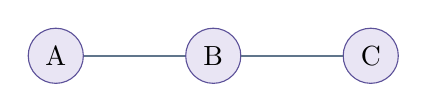
\begin{tikzpicture}[actor/.style={circle,draw=accent,fill=pale,minimum size=7mm}]
\node[actor](A) at (0,0){A}; \node[actor](B) at (2,0){B}; \node[actor](C) at (4,0){C};
\draw[edge,thick](A)--(B)--(C);
\end{tikzpicture}
\end{center}
\[
A=\begin{pmatrix}0&1&0\\1&0&1\\0&1&0\end{pmatrix}
\qquad
A^2=\begin{pmatrix}1&0&1\\0&2&0\\1&0&1\end{pmatrix}.
\]
\begin{itemize}
\item A can get to C in two steps through B, even though A and C have no direct tie.
\item B can return to itself in two ways: through A or through C.
\end{itemize}

\note{31--32 min. Adapted from the three-node chain in the 2025 deck. Point to the top-right entry and centre diagonal entry. In the six-person graph the same operation counts A--C--D.}
\end{frame}

\begin{frame}{Walks, paths, and matrix powers}

\begin{itemize}
\item A \textbf{walk} follows adjacent ties and may repeat actors or edges.
\medskip\item A \textbf{path} does not repeat actors.
\medskip\item $(A^\ell)_{ij}$ counts length-$\ell$ walks, not necessarily paths.
\end{itemize}
\[A\!\to\! B\!\to\! A\quad\text{is a two-step walk, not a path.}\]
In our undirected graph, $(A^2)_{ii}=k_i$: one return walk through each neighbour.

\note{32--35 min. Use arrows here to show the order of traversal, not directed edges in the undirected graph. In a directed network diagonal A squared counts reciprocal return walks and need not equal degree.}

\end{frame}

\begin{frame}{Exercise: two-step counts}

\activity{HAND CALCULATION: 4 MINUTES}

\begin{center}\network{A/B,A/C,B/C,C/D,D/E}\end{center}
Without multiplying the whole matrix, find:
\[(A^2)_{AA},\qquad(A^2)_{AB},\qquad(A^2)_{AE}.\]
List the contributing walks. Can a zero entry in $A^2$ rule out a longer connection?

\note{35--39 min. Four minutes, individual then compare with a neighbour. Expected 2, 1, 0. A reaches E in three steps.}

\end{frame}

\begin{frame}{Answer: what a zero does and does not mean}

\begin{align*}
(A^2)_{AA}&=2&&\text{via A--B--A and A--C--A},\\
(A^2)_{AB}&=1&&\text{via A--C--B},\\
(A^2)_{AE}&=0&&\text{no two-step walk}.
\end{align*}
But A--C--D--E is a three-step path, so $(A^3)_{AE}\geq1$.
\medskip
\textcolor{accent}{A zero in one matrix power rules out one length, not all lengths.}

\note{39--42 min. For this graph A cubed at A,E is exactly one. Distinguish no tie, no walk of a particular length, and unreachable.}

\end{frame}

\begin{frame}{Reachability from matrix powers}

For distinct actors in a finite graph,
\[j\text{ is reachable from }i
\iff \sum_{\ell=1}^{n-1}(A^\ell)_{ij}>0.\]
\begin{itemize}
\item If any walk exists, a path exists after removing loops in the walk.
\medskip\item A path visits each actor at most once: its length is at most $n-1$.
\medskip\item This explains reachability; software usually uses graph-search algorithms.
\end{itemize}

\note{42--45 min. This is a statement for nonnegative binary adjacency, with reachability between distinct actors. Do not recommend computing huge matrix powers for large sparse networks: counts grow and numerical overflow becomes possible.}

\end{frame}

\begin{frame}{Shortest paths and geodesic distance}

\[d(i,j)=\min\{\ell\geq1:(A^\ell)_{ij}>0\}\qquad(i\ne j).\]
\begin{itemize}
\item Set $d(i,i)=0$.
\medskip\item If $j$ is unreachable from $i$, set $d(i,j)=\infty$.
\medskip\item Here $d(A,E)=3$ via A--C--D--E, but $d(A,F)=\infty$.
\end{itemize}
Unweighted distance counts ties. It does not measure physical distance or elapsed time.

\note{45--48 min. A shortest unweighted walk between distinct actors is a path: a repeated cycle could be removed to shorten it.}

\end{frame}

\begin{frame}{The distance matrix}

\[\Delta=\disto\]
\begin{itemize}
\item Symmetric here because the network is undirected.
\item Infinite entries record genuinely unreachable pairs in this graph.
\end{itemize}

\note{48--51 min. Use Delta to avoid confusing distance matrix with degree diagonal D in the appendix. Ask students to read C,E and E,C, then F,A. Infinity is not a missing-data code.}

\end{frame}

\begin{frame}{Connected components}

A component is a maximal set of actors connected by paths.
\begin{center}\network{A/B,A/C,B/C,C/D,D/E}\end{center}
\[\{A,B,C,D,E\}\qquad\text{and}\qquad\{F\}.\]
Reordering nodes by component makes $A$ block diagonal: no ties, and no walks, cross between blocks.

\note{51--54 min. Maximal means no further node can be added while preserving connection to the set. An isolate is a component of size one. Our node order already groups components, with a five-by-five block and a zero block.}

\end{frame}

\begin{frame}{Connectivity in a directed graph}

\begin{center}\network[-{Stealth[length=2mm]}]{A/B,A/C,B/C,C/D,D/E}\end{center}
\begin{itemize}
\item \textbf{Weak connectivity:} connected after ignoring directions.
\medskip\item \textbf{Strong connectivity:} each actor can reach every other in the set by following directions.
\end{itemize}
A can reach E; E cannot reach A. A--E form one weak component, but each actor is its own strong component.

\note{54--58 min. The graph is a directed acyclic nomination network. F forms its own weak and strong component. Advice-seeker to source arrows are nomination direction, not guaranteed direction of advice transmission.}

\end{frame}

\begin{frame}{Bridges and articulation points}

\begin{itemize}
\item A \textbf{bridge} is an edge whose removal increases the number of components.
\medskip\item An \textbf{articulation point} is a node whose removal increases the number of components.
\end{itemize}
\begin{center}\network{A/B,A/C,B/C,C/D,D/E}\end{center}
C--D and D--E are bridges; C and D are articulation points.

\note{58--62 min. Count all components, including F. Removing C creates AB, DE, and F: three instead of two. Removing D creates ABC, E, and F. E is a leaf, but not an articulation point. Definitions here are for the undirected graph.}

\end{frame}

\begin{frame}{Exercise: alternative routes}

\activity{PAIRS: 6 MINUTES}

Suppose we add B--D while retaining all original ties.
\begin{center}\network{A/B,A/C,B/C,C/D,D/E,B/D}\end{center}
\begin{enumerate}
\item Is C--D still a bridge?
\item Is C still an articulation point? What about D?
\item Which A-to-E shortest paths now exist?
\end{enumerate}

\note{62--68 min. Six minutes in pairs, including a quick check with another pair. Ask students to distinguish edge removal from node removal.}

\end{frame}

\begin{frame}{Answer: redundancy changes social position}

\begin{itemize}
\item C--D is no longer a bridge: C--B--D is an alternative route.
\medskip\item C is no longer an articulation point; D still separates E from the rest.
\medskip\item A--C--D--E and A--B--D--E are both shortest paths of length 3.
\end{itemize}
\medskip
C's degree stays 3, yet its exclusive brokerage disappears.
\textcolor{accent}{A position depends on the surrounding network, not only the actor's own ties.}

\note{68--75 min. Debrief for seven minutes, drawing the two routes. This anticipates the fractional counting rule in betweenness. B degree rises from two to three and D from two to three. F remains isolated.}

\end{frame}

\begin{frame}{Break}

\begin{center}\Large 15 minutes\end{center}

\note{75--90 min. Resume at minute 90. Ask students to keep the original graph handy for the centrality calculations.}

\end{frame}

\begin{frame}{Degree and its matrix form}

\[\mathbf{k}=A\ones,\qquad C_D(i)=\frac{k_i}{n-1}.\]
For the undirected graph:
\[\mathbf{k}=(2,2,3,2,1,0)^{\mathsf T}.\]
\begin{itemize}
\item Normalising divides by the largest possible degree.
\medskip\item C has $C_D(C)=3/5=0.6$.
\medskip\item Degree ignores indirect connections and alternative routes.
\end{itemize}

\note{90--92 min. Brief retrieval rather than reteaching class 1. These are binary loopless degree formulas; weights require strength.}

\end{frame}

\begin{frame}{Who can reach the group in fewer steps?}

\begin{center}\network{A/B,A/C,B/C,C/D,D/E}\end{center}
Compare C and D within the connected group A--E.
\begin{itemize}
\item C needs one step to A, B, and D, and two to E: \textbf{5 steps in total}.
\item D needs two steps to A and B, and one to C and E: \textbf{6 steps in total}.
\end{itemize}
\textbf{Closeness} rewards shorter distances to the rest of the group. C scores higher: $4/5$ versus $4/6$.

\note{92--95 min. Explain the numerator four: four other actors. The score is one divided by the average distance. Ask which actor might reach the connected group with fewer handoffs if each tie allows one handoff.}
\end{frame}

\begin{frame}{What should we do with F?}

Nobody in the connected group can reach F. There is no number of steps we can add for that trip.
\begin{itemize}
\item If our question is only about A--E, we can use closeness within that group.
\medskip\item If our question is about all six actors, dropping F changes the question.
\end{itemize}
\textcolor{accent}{Harmonic centrality gives credit for actors you can reach, and zero credit for actors you cannot.}

\note{95--97 min. Use F to motivate an alternative rather than introduce an infinity calculation. Software conventions for closeness differ. The notebook gives the exact formulas.}
\end{frame}

\begin{frame}{Nearby actors count more}

\begin{center}
\begin{tabular}{lccc}
\toprule
Distance & One step & Two steps & Unreachable\\\midrule
Credit & 1 & $1/2$ & 0\\\bottomrule
\end{tabular}
\end{center}
\begin{enumerate}
\item Give each other actor credit according to distance: at three steps, credit is $1/3$.
\item Add the credits and divide by the number of other actors, here five.
\end{enumerate}
This average is \textbf{harmonic centrality}. F stays in the comparison.

\note{97--100 min. Ask students to say the rule in words before applying it. The formula is the mean reciprocal distance to the other actors; unreachable actors contribute zero.}
\end{frame}

\begin{frame}{Exercise: compare distance-based positions}

\activity{HAND CALCULATION: 4 MINUTES}

Distances to the other five actors are:
\begin{center}\begin{tabular}{lccccc}
\toprule
Actor & \multicolumn{5}{c}{Distances to the others}\\\midrule
C & 1 & 1 & 1 & 2 & $\infty$\\
D & 2 & 2 & 1 & 1 & $\infty$\\
F & $\infty$ & $\infty$ & $\infty$ & $\infty$ & $\infty$\\\bottomrule
\end{tabular}\end{center}
Calculate normalised harmonic centrality for C, D, and F.
\medskip
Which of C and D has better distance-based access?

\note{100--104 min. Four minutes. Require the common denominator five. Tie meanings and model of travel still determine whether this structural advantage is relevant.}

\end{frame}

\begin{frame}{Answer: harmonic centrality}

\begin{align*}
C_H(C)&=\frac{1+1+1+1/2+0}{5}=0.7,\\[1ex]
C_H(D)&=\frac{1/2+1/2+1+1+0}{5}=0.6,\\[1ex]
C_H(F)&=0.
\end{align*}
C is closer to more actors. The calculation retains the unreachable actor rather than silently removing it.

\note{104--106 min. Explain that harmonic centrality differs from closeness even in connected graphs: sum of inverses versus inverse sum. Scores should not be numerically interchanged.}

\end{frame}

\begin{frame}{Who is on the route between others?}

\begin{center}\network{A/B,A/C,B/C,C/D,D/E}\end{center}
Suppose A needs to get a message to E. The shortest route is A--C--D--E.
\begin{itemize}
\item C and D each get one point for being between A and E.
\item A and E are the endpoints, so they do not score for this pair.
\end{itemize}
\textbf{Betweenness} repeats this across pairs. It describes potential brokerage when shortest routes matter.

\note{106--109 min. Ask students to trace the path and identify intermediaries before counting other pairs. Unreachable pairs contribute zero. The notebook includes the formal definition.}
\end{frame}

\begin{frame}{Counting C's betweenness}

\begin{center}\network{A/B,A/C,B/C,C/D,D/E}\end{center}
The pairs whose unique shortest route passes through C are
\[\{A,D\},\quad\{A,E\},\quad\{B,D\},\quad\{B,E\}.\]
Each contributes 1, so $B(C)=4$. Similarly, $B(D)=3$.
\medskip
Pairs involving F are unreachable and add nothing.

\note{109--112 min. D lies between A,E; B,E; and C,E. A,B are endpoints for some routes but never internal on a shortest route. Count explicitly rather than equating bridges with scores.}

\end{frame}

\begin{frame}{Equal shortest paths split the contribution}

\begin{center}
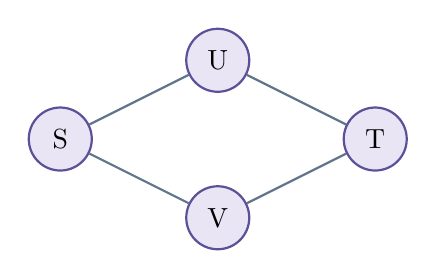
\begin{tikzpicture}[actor/.style={circle,draw=accent,fill=pale,minimum size=8mm},every path/.style={draw=edge,thick}]
\node[actor](S) at (0,0){S};\node[actor](U) at (2,1){U};\node[actor](V) at (2,-1){V};\node[actor](T) at (4,0){T};
\draw(S)--(U)--(T);\draw(S)--(V)--(T);
\end{tikzpicture}\end{center}
Two shortest S-to-T paths exist: S--U--T and S--V--T.
\[\frac{\sigma_{ST}(U)}{\sigma_{ST}}=\frac12,\qquad
\frac{\sigma_{ST}(V)}{\sigma_{ST}}=\frac12.\]
These are contributions from one pair, not the actors' full betweenness scores.

\note{112--114 min. Make clear this separate diamond graph illustrates counting only; node labels differ from the main graph. Avoid reporting U or V total betweenness as one half without including all pairs.}

\end{frame}

\begin{frame}{What does a betweenness score of 4 mean?}

C lies on the shortest routes of four pairs. Is four a lot?
\begin{itemize}
\item In this graph there are five other actors, making ten possible pairs that do not include C.
\medskip\item C's score of four is therefore $4/10=0.4$ of the maximum possible score.
\medskip\item Pairs involving F count among those ten possibilities, even though none can use C.
\end{itemize}
\textcolor{accent}{Say which actors were included before comparing scores.}

\note{114--116 min. The denominator is the number of unordered pairs excluding the focal actor. The exercise keeps F in the population.}
\end{frame}

\begin{frame}{Different measures describe different positions}

\begin{center}\begin{tabular}{lrrr}
\toprule
Actor & Degree & Harmonic & Betweenness\\\midrule
A & 2 & .567 & 0\\
B & 2 & .567 & 0\\
C & 3 & .700 & 4\\
D & 2 & .600 & 3\\
E & 1 & .433 & 0\\
F & 0 & .000 & 0\\\bottomrule
\end{tabular}\end{center}
A and D have equal degree. D is on more shortest routes and is a little closer to the rest of the group.
\medskip
{\footnotesize Harmonic normalised by $n-1$; betweenness raw.}

\note{116--119 min. Values checked in igraph. Different columns have different scales; compare actors within columns, not numerical values across columns.}

\end{frame}

\begin{frame}{Which position matters for your question?}

\begin{itemize}
\item Reaching many direct collaborators: consider degree or strength.
\medskip\item Access through short routes: consider harmonic centrality.
\medskip\item Connecting otherwise separated circles: examine brokerage and alternative routes.
\end{itemize}
What additional evidence would you need before calling an actor ``influential''?

\note{119--122 min. Three-minute discussion. Require students to name a tie definition and a plausible process. Prestige as receiving nominations is not identical to contact volume.}

\end{frame}

\begin{frame}{Exercise: choose the measure before calculating}
\activity{PAIRS: 2 MINUTES}
For each question, choose a measure and explain one assumption.
\begin{enumerate}
\item Who has the largest number of direct collaborators?
\medskip\item Who connects groups through their shortest available routes?
\medskip\item Who is named as an advice source by the most people?
\end{enumerate}
\medskip
For advice nominations, arrows run from the seeker to the source.
\textcolor{accent}{For question 3, would you count incoming or outgoing ties?}
\note{122--124 min. Ask students to choose based on the actual question before seeing scores. Ask students to apply the measures just introduced and explain why direction matters for nominations.}
\end{frame}

\begin{frame}{Answer: a research question determines a measure}
\begin{enumerate}
\item \textbf{Degree:} counts distinct direct collaborators. Use strength if the question concerns interaction volume.
\medskip\item \textbf{Betweenness:} counts participation in shortest paths. This assumes shortest routes matter to the process.
\medskip\item \textbf{In-degree:} counts incoming advice nominations. Out-degree would count how many advice sources a person names.
\end{enumerate}
\medskip
No score alone establishes influence, expertise, or power.
\note{124--125 min. Accept bridge or articulation analysis as a complementary answer to question 2, especially if students interpret connects as indispensability rather than participation.}
\end{frame}

\begin{frame}{Weights can mean strength or distance}

\begin{itemize}
\item For shortest paths, weights must represent \textbf{costs or lengths}: larger means harder or farther.
\medskip\item Interaction frequency usually represents \textbf{strength}: larger means more frequent contact.
\medskip\item If appropriate, define a separate cost $\ell_{ij}=1/w_{ij}$ for $w_{ij}>0$.
\end{itemize}
\medskip
That conversion is a substantive assumption, not an automatic correction.
In igraph, \texttt{weights = NA} explicitly requests unweighted paths.

\note{125--130 min. Distance-based igraph measures use the weight attribute by default when present. PageRank and eigenvector centrality treat positive weights as strengths instead. Never blindly reuse interaction counts as distances. Sources: igraph betweenness, harmonic centrality, and PageRank documentation.}

\end{frame}

\begin{frame}{Same number of contacts, different contacts}

\begin{center}\network{A/B,A/C,B/C,C/D,D/E}\end{center}
A and D each have two contacts. Look at whom they know:
\begin{itemize}
\item A knows B and C. Both have several contacts.
\item D knows C and E. E has only one contact.
\end{itemize}
\textbf{Eigenvector centrality} gives more credit for ties to people who themselves score highly.

\note{130--133 min. Contrast this with betweenness: D can be a broker even though A has more highly scored contacts. Ask which actor might score higher and why.}
\end{frame}

\begin{frame}{Eigenvectors: multiplication preserves a line}
Collect the actor scores in $\mathbf{x}$:
\[A\mathbf{x}=\lambda\mathbf{x},\qquad\mathbf{x}\ne\mathbf{0}.\]
\begin{itemize}
\item $\mathbf{x}$ is an \textbf{eigenvector}; $\lambda$ is its \textbf{eigenvalue}.
\medskip\item The product stays on the same line as $\mathbf{x}$. With $\lambda>0$, it also points in the same direction.
\medskip\item For a connected undirected graph with nonnegative ties, centrality uses the positive leading eigenvector.
\end{itemize}
Scale is arbitrary: if $\mathbf{x}$ works, so does $c\mathbf{x}$ for $c>0$.
\note{133--134 min. Define the equation, then immediately use the visual on the next slide. Negative eigenvalues reverse direction but preserve the eigenvector line. Centrality uses the nonnegative leading scores rather than an arbitrary eigenvector. In our graph the isolate has score zero.}
\end{frame}

\begin{frame}{A geometric example of an eigenvector}
An illustrative linear map doubles the first coordinate:
\[M=\begin{pmatrix}2&0\\0&1\end{pmatrix}.\]
\begin{columns}[c]
\column{.49\textwidth}\centering
\textbf{An ordinary vector changes direction}
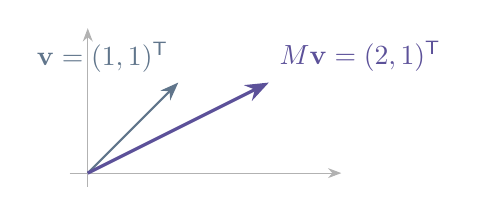
\begin{tikzpicture}[x=1.15cm,y=1.15cm,>=Stealth]
\draw[->,gray!60](-.2,0)--(2.8,0);\draw[->,gray!60](0,-.15)--(0,1.6);
\draw[->,edge,thick](0,0)--(1,1) node[above left] {$\mathbf{v}=(1,1)^{\mathsf T}$};
\draw[->,accent,very thick](0,0)--(2,1) node[above right] {$M\mathbf{v}=(2,1)^{\mathsf T}$};
\end{tikzpicture}
\column{.49\textwidth}\centering
\textbf{An eigenvector only changes length}
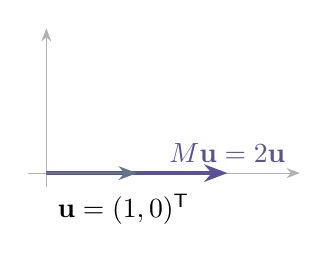
\begin{tikzpicture}[x=1.15cm,y=1.15cm,>=Stealth]
\draw[->,gray!60](-.2,0)--(2.8,0);\draw[->,gray!60](0,-.15)--(0,1.6);
\draw[->,accent,very thick](0,0)--(2,0) node[above] {$M\mathbf{u}=2\mathbf{u}$};
\draw[->,edge,thick](0,0)--(1,0);
\node[below] at (.85,-.12) {$\mathbf{u}=(1,0)^{\mathsf T}$};
\end{tikzpicture}
\end{columns}
\medskip
\textcolor{accent}{For $\mathbf{u}$, the eigenvalue is 2. Network centrality finds a corresponding direction in actor-score space.}
\note{134--136 min. M is an illustrative coordinate transformation, not the observed network adjacency. For v, the slope changes from 1 to one half. For u, the horizontal direction is preserved and the length doubles. In an n-actor network the vector has n coordinates; the same equation applies.}
\end{frame}

\begin{frame}{Give everyone a score, then look at their neighbours}

\begin{enumerate}
\item Start everyone at 1. Add up their neighbours' scores. This first round is just degree.
\medskip\item Now give each neighbour the score from the previous round. A adds B's 2 and C's 3; D adds C's 3 and E's 1.
\medskip\item A gets $2+3=5$; D gets $3+1=4$. They started with the same degree.
\end{enumerate}
Each round is another multiplication by $A$. Rescale the scores so that the largest stays at 1. In this network, the relative scores settle as we repeat.

\note{136--139 min. Show the unscaled second round before discussing rescaling. This follows the 2025 repeated-neighbour-update example. Ordinary iteration can oscillate on some graphs; see the appendix.}
\end{frame}

\begin{frame}{How do we know the scores have settled?}

On the scale where C scores 1, A scores about 0.82 and D about 0.57.
\begin{itemize}
\item Add each person's neighbours' scores one more time.
\medskip\item Every score is multiplied by roughly the same number, here 2.21.
\medskip\item Divide by that number and you recover the same relative scores.
\end{itemize}
\[A\mathbf{x}=\lambda\mathbf{x}.\]
That is the eigenvector equation: another round of neighbour scoring keeps the same relative positions.

\note{139--141 min. The notebook checks the numerical equation. Emphasise relative scores; 0.82 is not a probability or a share of all ties.}
\end{frame}

\begin{frame}{Who is nominating whom?}

In the directed advice network, A $\to$ B means A names B as an advice source.
\begin{itemize}
\item If we care about being named, we look at arrows pointing \emph{in}, not arrows pointing out.
\medskip\item The transpose turns the column of incoming nominations into a row we can use for scoring.
\medskip\item We can also ask how attention moves when people follow nomination arrows. PageRank takes this approach.
\end{itemize}

\note{141--143 min. Recall the earlier transpose example. Directed adjacency eigenvector centrality does not give a useful positive-eigenvalue ranking on this acyclic network; that detail is optional.}
\end{frame}

\begin{frame}{PageRank: follow the nominations}

Imagine moving from one actor to another by following their nominations.
\begin{itemize}
\item If A names two sources, choose each with probability one half.
\medskip\item If an actor names no one, choose a new actor at random.
\medskip\item Even when there are nominations to follow, occasionally jump to a random actor.
\end{itemize}
\textbf{PageRank} asks where you would spend your time if you kept doing this.

\note{143--144 min. Make clear that this is a model of following nominations, not a claim that advice itself flows from seeker to source.}
\end{frame}

\begin{frame}{A worked PageRank transition row}
A nominates B and C, so $k_A^{\mathrm{out}}=2$:
\[A_{A\cdot}=\begin{pmatrix}0&1&1&0&0&0\end{pmatrix}
\quad\Longrightarrow\quad
P_{A\cdot}=\begin{pmatrix}0&\tfrac12&\tfrac12&0&0&0\end{pmatrix}.\]
E has no outgoing ties; our dangling-node rule gives
\[P_{E\cdot}=\begin{pmatrix}\tfrac16&\tfrac16&\tfrac16&\tfrac16&\tfrac16&\tfrac16\end{pmatrix}.\]
\begin{itemize}
\item Both rows sum to 1; F receives the same uniform-row treatment as E.
\item At every actor, with probability $1-\alpha$, teleport using $\mathbf{v}=\ones/6$; otherwise follow $P$. Here $\alpha=0.85$.
\end{itemize}
\note{144--146 min. Read columns in actor order A--F. Ask where one unit at A goes before introducing teleportation: one half to B and one half to C. Uniform dangling redistribution is built into P; teleportation is a separate operation applied to every row. With teleportation, A's final transition probabilities are .45 each to B and C and .025 each to A, D, E, F. They sum to one.}
\end{frame}

\begin{frame}{Why PageRank can disagree with in-degree}

In our directed graph, C receives two nominations. E receives just one, from D.
\begin{itemize}
\item Following arrows can take you from A or B through C, then D, then E.
\medskip\item E's single nomination comes from D, an actor that already receives attention and sends all of its outgoing attention to E when following a tie.
\medskip\item In this example, E has the highest PageRank even though C has the highest in-degree.
\end{itemize}
\textcolor{accent}{In-degree counts nominations. PageRank also depends on where they come from and how attention is divided.}

\note{146--149 min. Use the diagram from directed connectivity. The notebook gives the scores and exact calculation. Explain that a different network or random-jump rule can change the rankings.}
\end{frame}

\begin{frame}{Linear algebra connects the measures}

\begin{center}\begin{tabular}{ll}
\toprule
Operation & Network interpretation\\\midrule
$A\ones$, $A^{\mathsf T}\ones$ & Out-degree, in-degree\\
$(A^\ell)_{ij}$ & Number of length-$\ell$ walks\\
First nonzero power at $(i,j)$ & Shortest unweighted distance\\
$A\mathbf{x}=\lambda\mathbf{x}$ & Undirected recursive centrality\\
Share attention along arrows & PageRank\\\bottomrule
\end{tabular}\end{center}
Harmonic centrality and betweenness use shortest-path information derived from the graph.

\note{149--150 min. One-minute recap. Avoid claiming all measures are simple matrix powers: betweenness also needs counts and participation of shortest routes.}

\end{frame}

\begin{frame}{igraph practical: start with the data}
Open \texttt{code/SNA\_Practical\_01\_02.Rmd} at the igraph introduction.
\begin{enumerate}
\item Build the advice network from a node table and a tie table.
\item Inspect direction, attributes, and isolates.
\item Rebuild it from its adjacency matrix and check that it matches.
\item Edit a copy and compare plots before calculating any scores.
\end{enumerate}
\note{150--152 min. Load igraph and run the running example. Keep g as the baseline. Work through the notebook's in-class blocks; extra import formats and cleaning examples are for reference afterward.}
\end{frame}

\begin{frame}[fragile]{From tables and matrices to graphs}
\begin{lstlisting}
g <- graph_from_data_frame(edges, directed = FALSE,
                           vertices = nodes)
V(g)$name
as_data_frame(g, what = "both")

A <- as_adjacency_matrix(g, sparse = FALSE)
g_matrix <- graph_from_adjacency_matrix(
  A, mode = "undirected", diag = FALSE)
\end{lstlisting}
Check the node IDs and direction. The node table keeps F even though F appears in no tie.
\note{152--159 min. Use the notebook to inspect node and edge attributes. Point out that V and E select vertices and edges. Match row and column order before importing a matrix. Compare the two graphs by their named adjacency matrices.}
\end{frame}

\begin{frame}[fragile]{Edit a copy and keep the layout fixed}
\begin{lstlisting}
g_added <- add_edges(g, c("B", "D"))
g_team <- induced_subgraph(g, c("A", "B", "C"))

set.seed(42)
xy <- layout_with_fr(g)
plot(g,       layout = xy)
plot(g_added, layout = xy)
\end{lstlisting}
The same actors stay in the same positions. What changed in the network?
\note{159--167 min. Show adding and deleting an edge, selecting an induced subgraph, and retaining the baseline graph. Use the notebook's team colours and contact widths to distinguish attributes from layout. Reuse coordinates only when the vertex order and set match.}
\end{frame}

\begin{frame}{Perturbation: add one alternative route}

\activity{PREDICT, THEN CHECK}

\begin{center}\network{A/B,A/C,B/C,C/D,D/E,B/D}\end{center}
\begin{itemize}
\item Predict C's degree and betweenness before recomputing.
\item Compare the changes for B, C, and D.
\item Does a high score identify an indispensable actor?
\end{itemize}

\note{167--172 min. Use the notebook’s “Add an alternative route: what changes?” section. C degree remains three; raw betweenness falls four to one. B becomes one, D remains three. Bridge and articulation-point status give a separate view of indispensability.}

\end{frame}

\begin{frame}{Interpret the results as a researcher}

Choose one actor and explain its position using two measures.
\begin{itemize}
\item State the tie definition and the population being analysed.
\medskip\item Explain the measures' different assumptions.
\medskip\item Identify one conclusion the scores do not support.
\end{itemize}
\medskip
Optional mathematical check: compare an eigenvector residual or manual PageRank with the package output.

\note{172--175 min. Pairs compare interpretations; discuss one example as a class. Do not require every pair to finish the PageRank extension within the session.}

\end{frame}

\begin{frame}{Exit question}

An actor's degree stays unchanged after a new tie is added between two other actors. Its betweenness falls sharply.
\begin{enumerate}
\item How can both statements be true?
\medskip\item Which feature of the surrounding network changed?
\medskip\item Why does $A^2$ count walks rather than only paths?
\end{enumerate}

\note{175--178 min. Three minutes individually. Use answers to assess whether students distinguish direct ties, alternative routes, and repeated actors.}

\end{frame}

\begin{frame}{What you should take away}

\begin{itemize}
\item Matrix products describe indirect routes and neighbour aggregation.
\medskip\item Connectivity determines which actors can reach one another.
\medskip\item Centrality measures capture different structural positions.
\medskip\item A new alternative route can change brokerage without changing degree.
\medskip\item Scores require a tie definition and a plausible social interpretation.
\end{itemize}

\note{178--180 min. 178--180: exit answer: the new edge provides an alternative route bypassing the actor; matrix multiplication permits repeated actors, such as A-B-A. Next class: collecting, preparing, and visualising empirical network data.}

\end{frame}

\begin{frame}{Reading and references}

\small
\begin{itemize}
\item Borgatti et al. (2022). \emph{Analyzing Social Networks Using R}. Mathematical foundations and chapters on node measures and centrality.
\medskip\item Kolaczyk \& Cs\'{a}rdi (2020). \emph{Statistical Analysis of Network Data with R}, 2nd ed. Chapters 2 and 4; selected mathematical-model sections.
\medskip\item Implementation details: \href{https://r.igraph.org/reference/harmonic_centrality.html}{harmonic centrality}, \href{https://r.igraph.org/reference/betweenness.html}{betweenness}, \href{https://r.igraph.org/reference/eigen_centrality.html}{eigenvector centrality}, and \href{https://r.igraph.org/reference/page_rank.html}{PageRank} in the igraph documentation.
\end{itemize}

\note{Reference slide outside the timed session. All plotted networks and numerical examples are synthetic. The notebook includes reproducible calculations and checks.}

\end{frame}

\appendix

\begin{frame}{Appendix: PageRank as a linear system}

For a column vector of probabilities $\mathbf{p}$,
\[\mathbf{p}=\alpha P^{\mathsf T}\mathbf{p}+(1-\alpha)\mathbf{v},
\qquad\sum_i p_i=1.\]
Rearrange:
\[\boxed{(I-\alpha P^{\mathsf T})\mathbf{p}=(1-\alpha)\mathbf{v}.}\]
\begin{itemize}
\item $I$ leaves a vector unchanged: $I\mathbf{p}=\mathbf{p}$.
\item $0<\alpha<1$ and positive uniform teleportation give a unique probability vector.
\end{itemize}

\note{Optional. Show that an n-by-n matrix multiplies an n-by-one vector on both sides. Notebook solves this system and compares with igraph. It is not necessary to compute an explicit matrix inverse. Source: https://r.igraph.org/reference/page_rank.html.}

\end{frame}

\begin{frame}{Appendix: the graph Laplacian}

For an undirected graph, let $D=\operatorname{diag}(k_1,\ldots,k_n)$.
\[L=D-A,\qquad L\ones=\mathbf{0}.\]
For actor $i$,
\[(L\mathbf{x})_i=k_ix_i-\sum_j A_{ij}x_j
=\sum_j A_{ij}(x_i-x_j).\]
The result compares the actor's value with its neighbours' values.
\medskip
The number of zero eigenvalues of $L$ equals the number of connected components.

\note{Optional extension, not part of the 180 minutes. For the six-node graph there are two zero eigenvalues. Use D for the degree diagonal and Delta for distances. This is for undirected graphs with nonnegative weights.}

\end{frame}

\begin{frame}{Appendix: a quadratic form measures disagreement}

For the unweighted undirected graph,
\[\mathbf{x}^{\mathsf T}L\mathbf{x}
=\frac12\sum_{i,j}A_{ij}(x_i-x_j)^2
=\sum_{\{i,j\}\in E}(x_i-x_j)^2.\]
\begin{itemize}
\item Each edge contributes the squared difference between its endpoints.
\medskip\item If values are constant within every component, the expression is zero.
\medskip\item This links connectivity to smoothing and spectral methods.
\end{itemize}

\note{Optional. Binary values x=(0,0,0,1,1,0) give energy one because only C-D crosses between values. This connects later to community detection without deriving a clustering algorithm.}

\end{frame}

\begin{frame}{Appendix: structural equivalence}

Actors can have similar positions without being adjacent.
For distinct $i$ and $j$, compare ties to all other actors:
\[A_{ik}=A_{jk}\quad\text{for all }k\notin\{i,j\}.\]
For directed data, compare incoming ties as well.
\medskip
In our undirected network, A and B have identical ties to everyone outside their pair. Interchanging A and B leaves the graph unchanged.
\medskip
\textcolor{accent}{Centrality describes a score; equivalence compares patterns of relations.}

\note{Optional sociological extension. The pair-excluded definition accommodates adjacent actors; strict full-row equality would fail due to the diagonal and mutual edge entries. Distinguish structural equivalence from looser role or regular equivalence.}

\end{frame}

\begin{frame}{Appendix: a stable power iteration}

On a connected undirected graph with at least one edge, use
\[\widetilde{\mathbf{x}}^{(t+1)}=(A+I)\mathbf{x}^{(t)}\]
followed by normalisation.
\begin{itemize}
\item If $A\mathbf{x}=\lambda\mathbf{x}$, then $(A+I)\mathbf{x}=(\lambda+1)\mathbf{x}$.
\medskip\item Eigenvectors are unchanged; eigenvalues shift by 1.
\medskip\item The positive diagonal prevents the bipartite oscillation of ordinary adjacency power iteration.
\end{itemize}

\note{Optional extension. This is a numerical device, not a substantive claim that the observed graph has self-ties. With the full disconnected six-node graph, the nontrivial component still dominates the isolate. Notebook uses the shift as an optional robustness check.}

\end{frame}

\end{document}
